
\section{Bayesian Neural PBC}

In this section, we present a unified framework that simultaneously combines
the \textsc{NeuralPbc} technique and rigorously addresses model uncertainties using
Bayesian learning.
%
Motivated by~\cite{sirichotiyakul2020data}, we incorporate uncertainties into
the dynamics and cast the passivity-based control synthesis problem as a
stochastic optimization problem.
%
The closed-loop storage (energy-like) function, from which the control law is
derived, is not restricted to a certain form and instead represented by a neural
network whose parameters are random variables.
%
% The second aim is to develop an algorithm that find a suitable family of
% parameters for the energy-like function such that the behavior of the
% closed-loop trajectories optimizes a certain performance objective.
%
We apply Bayesian learning and develop an algorithm that finds a suitable
probability distribution of the neural net parameters automatically.
%
In contrast to deterministic optimization, this approach provides a probability
distribution over the neural net parameters instead of a point estimate,
providing a way to reason about model uncertainties and measurement noise during
the learning process.
%
We demonstrate the efficacy and robustness of our current framework with a
comparison against the deterministic framework~\cite{sirichotiyakul2020data}.
The comparison is performed on benchmark underactuated control problems--the
simple pendulum and the inertia wheel pendulum--both in simulation and
real-world experiments. 
%

\subsection{Control Design for Smooth Dynamical Systems}
\label{ssec:pbc_smooth_dynamics}

In this section, we formulate the Bayesian learning framework that minimizes
the effects of system parameter uncertainties and measurement errors for smooth dynamical systems. 
%
In this framework, the neural net parameterization of $H^\theta_d$ given in
Section~\ref{ssec:pbc} is replaced by a Bayesian neural
network whose weights and biases are samples drawn from a posterior distribution.
%
The goal is to learn this posterior that achieves the performance objective under system parameter and measurement uncertainties. 
%


Let $\phi(x_0, u^\theta, T)$ denote a closed loop trajectory integrated from the Hamilton's equation of motion in~\eqref{eq:hamiltonian_dynamics}.
The trajectory starts from the initial state $x_0$ and spans for the time horizon $T$.
%
We sample the initial state $x_0$ through greedy and explorative state sampling techniques discussed in Section~\ref{sssec:state_sampling}.
The control law $u^\theta$ consists of the energy shaping and damping terms found from the desired Hamiltonian $H^\theta_d$ as shown in equation~\eqref{eq:damping_and_es_control}.
%
To generate this trajectory, we first sample the parameters $\theta$ from the prior distribution $P(\theta)$.
%

We take two approaches to selecting the prior distribution.
The simplest approach is to use an uninformed prior given by a uniform distribution;
this choice encourages
exploration but has slow convergence properties. The second approach uses an
informed prior that warm-starts the Bayesian training around the solution of the
deterministic training. To do so, the prior
distribution is a Gaussian probability distribution centered around the parameters learned from the deterministic
\textsc{NeuralPbc} technique discussed in Section~\ref{ssec:pbc}.

With the trajectories generated from the prior distribution samples, we compose a performance objective as follows.
\begin{align*}
    J(\phi, u) = \mathbb{E}_{x_0 \sim \mathcal{D}_N}[ \ell(\phi(x_0, u, T), u)], 
\end{align*}
\noindent where $\mathcal{D}_N$ is a collection of initial states sampled with explorative and greedy state sampling techniques (Section~\ref{sssec:state_sampling}), and
$\ell$ is the running cost of the trajectories. We provide three options for the running cost in the next section.
%
In order to update the posterior distribution based on the performance of the generated trajectories, we compose the likelihood function as
\begin{align}
    P(J \mid \theta) = \mathcal{N}\left(0, s \right), 
    \label{eqn:likelihood_neuralpbc}
\end{align}
\noindent where $s$ is the standard deviation of the likelihood.
%
Notice that the likelihood is maximum when the expectation of the running cost $J$ is minimum.
%
\begin{rem}
    On top of the neural net parameters $\theta$, we can learn the posterior
    over the standard deviation $s$ of the likelihood. 
    This automatically finds the weighting between the likelihood and prior distributions, achieving optimal \textit{bias-variance trade-off}.
    In this scenario, the posterior distribution is a multivariate probability distribution over the parameters $\theta$ and $s$. 
\end{rem}

From here, we can use Hamiltonian Monte Carlo or variational inference (Section~\ref{ssec:bayesianLearning}) to find the posterior distribution from the likelihood and the prior.
%
We first pose the search over the posterior as the following optimization problem.
\begin{equation}
    \begin{aligned}
        \underset{P(\theta | J)}{\textrm{minimize}} 
        & & J(\phi, u) &= \mathbb{E}_{x_0 \sim \mathcal{D}_N}[ \ell(\phi(x_0, u, T), u)]  , \\
        \textrm{subject to}
        & & \bmat{\dot{q} \\ \dot{p}} &= \bmat{\phantom{-}\nabla_p H \\ -\nabla_q H} + \bmat{0 \\ \Omega(q)}u^{\theta}, \\%
        & & u^{\theta} &= -\Omega^{\dagger} (\nabla_q H_d^{\theta} - \nabla_q H), \\
        & & p_s &\sim \mathcal{N}(\hat{p}_s, \sigma_p), \\
        & & \theta &\sim P(\theta | J).
    \end{aligned}
    \label{eq:smooth_bayesian_pbc}
\end{equation}
We expand on the use of HMC and variational inference to solve the optimization problem.
%
\begin{enumerate}
    \item \textbf{Hamiltonian Monte Carlo (HMC)}: represents the posterior with a large collection of samples denoted by $\Theta$.
    %
    We draw the first sample $\theta^{(\tau=0)}$ from the prior distribution and construct the likelihood from the performance objective as $P(J | \theta^{(\tau=0)})$.
    %
    The likelihood and the prior distributions are known in closed form, hence the joint distribution $P(\theta^{(\tau=0)}, J)$ is given by
    \begin{align*}
        P(\theta^{(\tau=0)}, J) = P(J|\theta^{(\tau=0)})P(\theta^{(\tau=0)}).
    \end{align*}
    We generate the next sample from a Markov Chain, which is given the following first order differential equations~\cite{bishop2006pattern}
    %
    % The Markov Chain is constructed from two coupled first order differential equations, taken from the classical dynamics of a particle in motion.
    \begin{equation}
        \begin{gathered}
            m^{\tau + \nicefrac{\Delta \tau}{2}} = m^{\tau} - \dfrac{\Delta \tau}{2} \dfrac{\partial P(\theta^{\tau}, J)}{\partial \theta^{\tau}} \\
            \theta^{\tau + \Delta \tau} = \theta^{\tau} + m^{\tau + \nicefrac{\Delta \tau}{2}} \; \Delta t \\
            m^{\tau + \Delta \tau} = m(\tau + \nicefrac{\Delta \tau}{2}) - \dfrac{\Delta t}{2}\dfrac{\partial P(\theta^{\tau + \Delta \tau}, J)}{\partial \theta^{\tau + \Delta \tau}}
        \end{gathered}
        \label{eq:leapfrog}
    \end{equation}

    %
    \noindent where $\tau=0$ for the first sample and $\Delta \tau$ is the integration time step. 
    This integration is commonly known as \textit{leap frog discretization}.
    %
    We accept or reject the sample $\theta^{\tau + \Delta \tau}$ based on the rule:
    \begin{align*}
        \nu &\sim \mathcal{U}(0, 1), \\
        A(\theta^{(\tau + \Delta \tau)}, \theta^{(\tau)}) &= \min \Biggl(1, \frac{P(\theta^{(\tau + \Delta \tau)}, J)}{P(\theta^{(\tau)}, J)} \Biggr),
    \end{align*} 
    If $A(\theta^{(\tau + \Delta \tau)}, \theta^{(\tau)}) \geq \nu$, then we accept the sample. 
    %
    Otherwise, we discard the candidate and resample from the prior distribution.
    %
    The complete procedure is outlined in Algorithm~\eqref{algo:hmc}
    %
    We keep collecting these samples until the average accumulated loss converges to the minimum achievable value. 

    Once we obtain the collection samples, we use them to evaluate the controller as follows.
    %
    From the collection $\Theta$, we sample $N_Q$ parameters in a uniform fashion.
    %
    We evaluate the neural net $H^\theta_d$ and the corresponding energy shaping and damping control for each sample.
    %
    Then, we marginalize over the control law as 
    \begin{equation*}
        u(x) = \frac{1}{N_Q} \sum_{\theta \sim P(\theta | J)} u(x; \theta).
    \end{equation*} 
    We repeat this computation for every state in a trajectory.

    \begin{algorithm}[H]
        \centering
        \setstretch{1.5}
        \caption{Bayesian \textsc{NeuralPbc} via Hamiltonian Monte Carlo}\label{algo:hmc}
        \begin{algorithmic}[1]
        \State $\Theta \leftarrow \{\}$ \Comment{Collection of samples}
        \State Define prior $P(\theta)$
        \While {$i < \texttt{maximum iteration}$}
            \State $\tau=0, \theta^{0} \sim P(\theta)$, $m^0 = 0$, accepted=true
            \While{accepted}
                \State $\mathcal{D}_N \gets \{x_0\}_{(N_{\mathcal{D}})}$  \Comment{$N_{\mathcal{D}}$ initial state samples}           
                \State $p_s \sim \mathcal{N}(\hat{p}_s, \sigma_p)$\Comment{Sample a system parameter}
                % \State $J(\phi, u) = \mathbb{E}_{x_0 \sim \mathcal{D}_N}[ \ell(\phi(x_0, u^{\theta^{\tau}}, T), u^{\theta^{\tau}})]$\Comment{Performance of current parameter}
                \State $J^\tau \leftarrow 0$,  $J^{\tau + \Delta \tau} \leftarrow 0$
                \For{$(x_0) \sim \mathcal {D}_N$}
                    \State $\phi \leftarrow \phi(x_0, u^{\theta^{\tau}}, T) $\Comment{Generate trajectory}
                    \State $J^\tau  \gets J^\tau  + \ell(\phi; \theta^{\tau})/N_{\mathcal{D}}$ \Comment{Batch loss of current parameter}
                \EndFor
                % \State $P(\theta^{(\tau)}, J) = P(J|\theta^{(\tau)})P(\theta^{(\tau)})$
                \State $m^{\tau + \Delta \tau}, \theta ^{\tau + \Delta \tau} \leftarrow \texttt{leap frog discretization}(m^{\tau}, \theta ^{\tau} )$\Comment{Equation~\eqref{eq:leapfrog}}
                % \State $m^{\tau + \nicefrac{\Delta \tau}{2}} = m^{\tau} - \dfrac{\Delta \tau}{2} \dfrac{\partial P(\theta^{\tau}, J)}{\partial \theta^{\tau}} $ \Comment{Generate Markov Chain}
                % \State $\theta^{\tau + \Delta \tau} = \theta^{\tau} + m^{\tau + \nicefrac{\Delta \tau}{2}} \; \Delta t $\Comment{Evaluate next parameter}
                % \State $m^{\tau + \Delta \tau} = m(\tau + \nicefrac{\Delta \tau}{2}) - \dfrac{\Delta t}{2}\dfrac{\partial P(\theta^{\tau + \Delta \tau}, J)}{\partial \theta^{\tau + \Delta \tau}}$
                % \State $J(\phi, u) = \mathbb{E}_{x_0 \sim \mathcal{D}_N}[ \ell(\phi(x_0, u^{\theta^{\tau + \Delta \tau}}, T), u^{\theta^{\tau + \Delta \tau}})]$\Comment{Performance of next parameter}
                \For{$(x_0) \sim \mathcal {D}_N$}
                    \State $\phi \leftarrow \phi(x_0, u^{\theta^{\tau + \Delta \tau}}, T) $\Comment{Generate trajectory}
                    \State $J^{\tau + \Delta \tau}  \gets J^{\tau + \Delta \tau}  + \ell(\phi; \theta^{\tau + \Delta \tau})/N_{\mathcal{D}}$ \Comment{Batch loss of next parameter}
                \EndFor
                % \State $P(\theta^{(\tau + \Delta \tau)}, J) = P(J|\theta^{(\tau + \Delta \tau)})P(\theta^{(\tau + \Delta \tau)})$
                \State $\nu \sim \mathcal{U}(0, 1)$
                \State $A(\theta^{(\tau + \Delta \tau)}, \theta^{(\tau)}) = \min \Biggl(1, \dfrac{P(\theta^{(\tau + \Delta \tau)}, J^{(\tau + \Delta \tau)})}{P(\theta^{(\tau)}, J^{(\tau)})} \Biggr)$
                \If {$A(\theta^{(\tau + \Delta \tau)}, \theta^{(\tau)}) \geq \nu$}
                    \State $\Theta$ \leftarrow \; $\Theta \cup \theta^{(\tau + \Delta \tau)}$ \Comment{Accept sampled parameter}
                    \State $\tau = \tau + \Delta \tau$
                    \Else
                    \State $i \leftarrow i + 1$, accepted=false\Comment{Reject sampled parameter}
                \EndIf
            \EndWhile
        \EndWhile
        \State \textbf{Return} $\Theta$
        \end{algorithmic}
    \end{algorithm}

    \item \textbf{Variation Inference (VI)}: intends to learn the distribution parameters $z$ of the pre-selected (approximate) posterior $Q(\theta; z)$.
    %
    Unlike HMC, we have a closed form probability distribution for the posterior.
    We draw several samples from the current posterior and evaluate its performance through the joint distribution $P(\theta, J)$. 
    Given the likelihood and the prior distributions, variational inference constructs the \textsc{Elbo} as
    \begin{align}
        \mathcal{L}(J,z) = \mathbb{E}_{\theta \sim Q} \left[\log(P(J | \theta)P(\theta)) - \log(Q(\theta;z)) \right].    \\
        \label{eq:neuralpbc_elbo}    
    \end{align}
    We use stochastic gradient descent to iteratively update the distribution parameteres as follows:
    \begin{align*}
      z \leftarrow z + \frac{ \partial \mathcal{L}(J,z)}{\partial z}
    \end{align*}
    The full variational inference training process is shown in Algorithm~\eqref{algo:vi}.
    
    The gradient ${\partial \mathcal{L}}/{\partial z}$ holds a rather complex form for two reasons.
    First, the \textsc{Elbo} is evaluated from trajectories integrated from the differential equations in~\eqref{eq:hamiltonian_dynamics}.
    We use a combination of adjoint method and auto-differentiation techniques~\cite{chen2018neural} to compute the
    gradient ${\partial \mathcal{L}}/{\partial z}$ through the trajectories.
    %
    Secondly, computing ${\partial \mathcal{L}}/{\partial z}$ requires the derivative
    of the sample $\theta$ with respect to the distribution parameters $z$, which is
    intractable. We handle this complication by invoking the reparameterization
    trick of the Automatic Differentiation Variational
    Inference(\textsc{ADVI})~\cite{kucukelbir2015automatic}.

    \begin{algorithm}
        \setstretch{1.2}
        \caption{Bayesian \textsc{NeuralPbc} via variational inference}
        \label{algo:vi}
        \small
        \begin{algorithmic}[1]
            \algrenewcommand\algorithmicindent{0em} % No indent
            \State $\mathcal{D}_N \gets \{x_0\}_{(N_{\mathcal{D}})}$  \Comment{$N_{\mathcal{D}}$ initial state samples} 
            \algrenewcommand\algorithmicindent{1.1em} % Change indent back to default
            \While{$i < $ \texttt{maximum iteration}}
            \State $\mathcal{L} \gets 0$ \Comment{\textsc{Elbo} Loss}
            \For{$i=1:Q_N$} \Comment{Samples to compute~\eqref{eq:neuralpbc_elbo}}
            \State $J \gets 0$ \Comment{Batch loss}
            \State $\theta \sim Q(\theta; z)$ \Comment{Sample parameters of $H^\theta_d$}
                \For{$(x_0) \sim \mathcal {D}_N$}
                \State $p_s \sim \mathcal{N}(\hat{p}_s, \sigma_p)$\Comment{Sample a system parameter}
                \State $\phi \leftarrow \phi(x_0, u, T) $\Comment{Generate trajectory}
                \State $J \gets J + \ell(\phi; \theta)/N_{\mathcal{D}}$ 
                \EndFor
            \State $\mathcal{L} \gets \mathcal{L} + \frac{1}{Q_N} \left(\log[P(J | \theta) P(\theta)] - \log[Q(\theta;z)]\right)$
            \EndFor
            \State $z \gets z + \alpha_i \nicefrac{\partial \mathcal{L}}{\partial z}$\Comment{SGD step}
            \State $\mathcal{D}_N \gets \{x_0\}_{(N_{\mathcal{D}})}$\Comment{New initial state samples}
            \State $i \;\:\gets i + 1$
            \EndWhile
            \State \textbf{return} $z$
        \end{algorithmic}
    \end{algorithm}
  
    \end{enumerate}

\subsubsection{Cost Function}
\label{sssec:cost}

The cost function $J$ helps impose various desired behaviors in the learned
controller. In this section, we present three performance objectives, their
corresponding likelihood functions and the desired behavior they impose.

\begin{enumerate}
    \item Trajectory tracking: Let $x^\star$ denote the desired equilibrium of a
    dynamical system and $\phi(x_0, u^\theta, T)$ represent a
    prediction from the initial condition $x_0$ with the current control law
    $u^\theta$. The objective of this task is to find a closed-loop controller
    that can track an expert trajectory $\phi^\star$ obtained from a path
    planner. To impose this behavior, the running cost is a function of the
    distance from the current trajectory $\phi$ to $\phi^\star$, defined in
    terms of the transverse coordinates $\phi_\bot-\phi^\star_\bot$ along
    the preferred orbit, using the ideas outlined
    in~\cite{shiriaev2009transverse,manchester2010transverse}. In this setting,
    the prediction converges to $\phi^\star$ if and only if
    $\phi_\bot-\phi^\star_\bot \xrightarrow{t \to \infty}{} 0$. In order to
    encourage this behavior, we define the cost function as
    %
    \begin{equation}
        % J_{\textrm{MSE}} =  \frac{1}{N} \sum_{n=0}^N \Big( \norm{x(t_n) - \hat{x}(t_n)}{} + \norm{u(t_n) - \hat{u}(t_n)}{} \Big)
        J_{track}(\phi_\bot) =  \sum_{x_\bot \in \phi_\bot, \; x^\star_\bot \in \phi^\star_\bot} |\left| x_\bot-x^\star_\bot | \right |^2
        \label{eq:xperploss}   
    \end{equation}
    %
    Thus, the likelihood can be constructed to minimize the cost $J_{track}$ as follows.
    \begin{align}
        P(J_{track} | \theta) = \prod_{x_\bot \in \phi_\bot, \; x^\star_\bot \in \phi^\star_\bot}\mathcal{N}(x^\star_\bot , s),
        \label{eq:track_likelihood}
    \end{align}
    %
    % where $\Sigma$ parameterizes the variance of the likelihood. On top of the
    % decision parameters $\theta$, we wish to learn the posterior over the
    % variance $\Sigma$ of the likelihood. This allows us to adaptively tune the
    % weights on the components of $x_\bot-x^\star_\bot$ on the overall cost, such
    % that we achieve optimum trajectory tracking. This is most advantageous when
    % the states of a system have high variance and the weights on
    % $x_\bot-x^\star_\bot$ need to be selected in such a way that one state does
    % not dominate the cost $J_{track}$.
    % %
    % Hence, the posterior distribution $p(\theta | \mathcal{D})$ is a multivariate
    % probability distribution over random variable $\xi$, where $\xi = [\theta,
    % \Sigma]$.
    \item Set distance loss: Let $\mathcal{S}$ represent a small convex
    neighborhood containing $x^\star$. The objective is to find a policy that
    pulls trajectories to the goal set $\mathcal{S}$. The cost function suitable
    for this task is set distance, $J_{\textrm{set}}$, between the current
    prediction $\phi$ and the goal set $\mathcal{S}$:
    %
    \begin{equation}
        J_{\textrm{set}}(\phi)
        = \underset{t}{\textrm{inf}} \, {\{ \norm{a - b}{}: a \in \phi(t),\, b \in \mathcal{S} \}}.  
        \label{eq:set_distance}
    \end{equation}
    % 
    For instance, the set $\mathcal{S}$ may be chosen as a ball of radius
    $r$ around $x^\star$ in the standard norm topology. 
    %
    Here, $r$ becomes a hyperparameter of the training algorithm. With a
    particular choice of $\mathcal{S}$, if at any point along the prediction
    $\phi$, a state $x$ is closer than $r$ to $x^\star$, no penalty is
    incurred by $J_{\textrm{set}}$. The corresponding likelihood function is
    given by 
    \begin{align}
        P(J_{\textrm{set}} | \theta) = \mathcal{N}(0, s).
        \label{eq:set_likelihood}
    \end{align}
    % where $s$ is a hyperparameter that represents the standard deviation of the
    % likelihood.
    %
    \item Terminal loss: encourages trajectories to remain as close to the
    desired state as possible at time $T$. Terminal loss, $\ell_T$, is the
    distance between the final state of the prediction $\phi$ and $x^\star$,
    which is given by
    %
    \begin{equation}
        J_T(\phi) = \ell_{\textrm{set}}(\phi) + \ell_T\left(\phi\right).
        \label{eq:nn_controller_j} 
    \end{equation}
    %
    The corresponding likelihood function is given by 
    \begin{align}
        P(J_T | \theta) = \mathcal{N}(0, s).
        \label{eq:terminal_likelihood}
    \end{align}
\end{enumerate}

\subsubsection{Uncertainty Modelling}

In Section~\ref{sec:bl_justification}, we have shown the deteriorated performance caused by system model discrepancies.
%
Moreover, in Section~\ref{ssec:bayesianLearning}, we have discussed how the variance in the stochastic control can prevent the Bayesian training from overfitting on inaccurate observations.
%
In this section, we give more structure to the desired variance of the Bayesian control.
%
We rigorously model the system parameter and measurement uncertainties of the system in order to guide the variance of the controller.
%
Hence, in the Bayesian framework, we inject these uncertainties directly into
the training loop in order to learn a controller that works for a wide range of
system parameters and measurement noise.
%
We model system parameter uncertainties by sampling a set of system parameters
$\zeta$ from a normal distribution $\mathcal{N}(\zeta_0, \sigma_{\zeta})$
centered around a nominal parameter $\zeta_0$.
%
Each time we generate a new trajectory starting from the initial states drawn
from the replay buffer $\mathcal{D}$, we draw a new sample of $\zeta$.
%


Additionally, we model measurement error by injecting noise into the prediction
$\gamma$.
%
This is achieved by replacing the dynamical constraint given
in~\eqref{eq:neural_pbc_finite_optim} with the following stochastic differential
equation (SDE).
\begin{align}
    \dd x &= \left(\bmat{\phantom{-}\nabla_p H \\-\nabla_q H} + \bmat{0 \\ G(q)}u^{\theta}(x) \right) \dd t + \nabla_x u(x) \dd W_t, 
    \label{eq:sde_initial}
\end{align}
where $\dd W_t$ is a correlated noise process, such as Wiener process, on the
states due to measurement uncertainties, and $\nabla_x u(x)$ is the coefficient
of the first-order Taylor approximation of $u^{\theta}(x)$ around zero noise. 

\begin{equation}
    \begin{aligned}
        \underset{P(\theta | J)}{\textrm{minimize}} 
        & & J(\phi, u) &= \mathbb{E}_{x_0 \sim \mathcal{D}_N}[ \ell(\phi(x_0, u, T), u)]  , \\
        \textrm{subject to}
        & & \dd x &= \left(\bmat{\phantom{-}\nabla_p H \\-\nabla_q H} + \bmat{0 \\ G(q)}u^{\theta}(x) \right) \dd t + \nabla_x u(x) \dd W_t, \\
        & & u^{\theta} &= -\Omega^{\dagger} (\nabla_q H_d^{\theta} - \nabla_q H), \\
        & & p_s &\sim \mathcal{N}(\hat{p}_s, \sigma_p), \\
        & & \theta &\sim P(\theta | J).
    \end{aligned}
    \label{eq:smooth_bayesian_pbc}
\end{equation}

\begin{rem}
    Introducing uncertainties to the deterministic training finds a point
    estimate of the optimal controller parameter, which may be interpreted
    as the mean of the optimal posterior distribution that Bayesian learning
    provides. A point estimate of the learned parameters is prone to be
    biased (for example, if the uncertainty in system parameters is large,
    the optimal parameter $\theta$ for the true system parameter may be
    quite far from the deterministic solution). This bias-variance trade-off
    problem is alleviated by Bayesian inference which allows one to
    marginalize over the posterior parameter
    distribution~\cite{bishop2006pattern}.
\end{rem}


%%%%%%%%%%%%%%%%%%%%%%%%%%%%%%%%%%%%%%%%%%%%%%%%%%%%%%%%%%%%%%%%%
%%%%%%%%%%%%%%%%%%%%%%%%%%%%%%%%%%%%%%%%%%%%%%%%%%%%%%%%%%%%%%%%%


\subsection{Simple Pendulum}

The equation of motion of a simple pendulum with measurement noise is given by
%
\begin{equation}
    \dd x = \bmat{
        \dot{q} \\ 
        a \sin{(q)} + u^\theta(x)
    } \dd t+ \nabla_x u^\theta(x) \dd W_t,
    \label{eq:pendulum_sde}
\end{equation}
%
where $a=mgl/I$, $\dd W_t$ is the Wiener process, $x = (q,
\dot{q})$ is the state of the pendulum where $q = 0$ corresponds
to the upright position, and the control input $u$ is the torque generated by
the actuator. 
%
The torque \(u^\theta\) is limited by \(\abs{u} \leq u_{\textrm{max}}\).
%
The maximum torque $u_{\textrm{max}}$ available is such that the upward
equilibrium point cannot be reached by just rotating in one direction, as the
gravitational force overcomes the motor torque eventually. The controller has to
be clever enough to overcome gravitational forcing with a combination of
built-up momentum and torque bandwidth.

The objective of this case study is to stabilize the homoclinic orbit of the
pendulum whose single parameter $a$ has the nominal value $9.81$
\unit{$s^{-2}$}. To this end, we learn a target function that directly
parameterizes the controller $u^\theta$.

\subsubsection{Training} 
Algorithm~\ref{algo:hmc} is carried out with expert
trajectories generated by the vanilla energy-shaping control
(ESC)~\cite{underactuated}. The ESC takes the general form
%
\begin{equation}
    u^\theta(q, \dot{q}; \theta) = \theta_1 \dot{q} + \theta_2 \cos{(q)} \dot{q} + \theta_3 \dot{q}^3,
    \label{eq:pendulum_esc}
\end{equation}
%
where the weights $\{\theta_i\}_{i=1}^3$ satisfy $-\theta_1 = \theta_2 = 2a
\theta_3 < 0$ in the vanilla ESC. 

The running cost function is chosen to be the loss $J_{track}(\phi_\bot)$
from homoclinic orbit $\phi^\star$ provided in~\eqref{eq:xperploss}; the
corresponding likelihood is given by~\eqref{eq:track_likelihood}. We collect
dataset $\mathcal{D}$ of initial states sampled from the expert trajectory,
per the state sampling technique discussed in
Section~\ref{ssec:state_sampling}. For this particular experiment, we use
Hamiltonian Monte Carlo outlined in Algorithm~\ref{algo:hmc} to infer the
exact posterior distribution $p(\theta | \mathcal{D})$. We compare the
Bayesian policy with
the deterministic policy, which is simply given by the point-estimates of
the expert vanilla ESC in~\eqref{eq:pendulum_esc}~\cite{acc}.

\subsubsection{Simulation Tests} 
The homoclinic orbit of the pendulum is defined by the $2a$-level set of the
total energy $\mathcal{H} = \nicefrac{1}{2}\dot{q}^2 + a(1 +
\cos{q})$. Hence, an appropriate measure of the distance to the
homoclinic orbit is given by the absolute value $\bigl| \mathcal{\tilde{H}}
\bigr|$ of the error: $\mathcal{\tilde{H}} = \mathcal{H} - 2a$. We evaluate the
performance of a closed-loop system by recording the value $\zeta = \min \,
\bigl| \mathcal{\tilde{H}} \bigr|$, where the minimum is taken over the last $2$
seconds of a $10$-second-long trajectory.


We demonstrate the robustness of the Bayesian policy by comparing $\zeta$,
as a function of the system parameter $a$, with that of the deterministic
policy.
%
We also investigate the effects of the prior distribution of $\theta$ on the
performance of the controllers.
%
In particular, we examine a uniform prior and a Gaussian prior centered around
the deterministic solution of~\eqref{eq:pendulum_esc}.
%
The comparisons between the controllers from both cases are shown in
Figure~\ref{fig:bayes_compare}.
%

In addition to uncertainties in $a$, we test the deterministic and Bayesian
policies with measurement noise, modelled as a Wiener process with variance
$0.0005$ \unit{rad} in the $q$- and $0.05$ \unitfrac{rad}{s} in the
$\dot{q}$-directions.
%
These numbers are chosen to represent a typical error arising from an
optical encoder with a resolution of 2048 pulses per revolution and its naive
differentiation via backward difference.
%
To capture the influence of measurement noise, we generate 20 trajectories
by integrating~\eqref{eq:pendulum_sde} from the same initial states. 
%
These trajectories are then used to compute $\zeta$. 
%
The effects of noise on $\zeta$ are reflected by the error bands in
Figure~\ref{fig:bayes_compare}.

The results show that Bayesian learning yields controllers that outperform 
their deterministic counterpart throughout the whole range of $a$.
%
The marginalization method in~\eqref{eqn:marginalization} for selecting $\theta$
from the learned distribution performs best when a uniform prior is used, while
the MAP method performs best with the Gaussian prior.
%
We emphasize that the error bands of the marginalized and MAP point
estimates stay well below those of the deterministic curve in the top plot of
Figure~\ref{fig:bayes_compare}.
%
This implies that the controllers produced by Bayesian learning perform
consistently better than the deterministic controller, demonstrating their
robustness against model uncertainty and measurement noise.


\begin{figure}[tb]
    \centering
    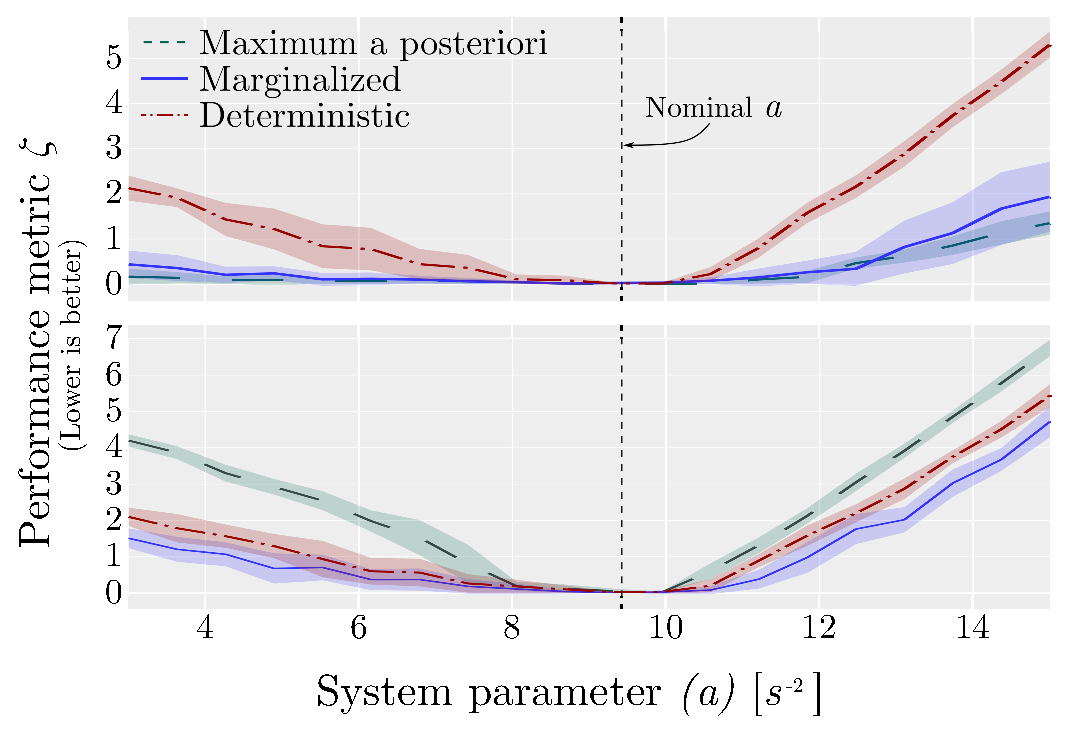
\includegraphics[width=0.7\linewidth]{figures/H_combined.eps}
    \caption{
        Performance comparisons between deterministic and Bayesian learning
        methods. 
        %
        The training is initialized with a Gaussian prior (top), and a
        uniform prior (bottom). 
        %
        The continuous error band is generated by computing $\zeta$ from 20
        trajectories of~\eqref{eq:pendulum_sde}, starting at the downward
        equilibrium with a small disturbance. 
        %
        The solid lines represent the mean of $\zeta$. 
        %
        Best viewed in color.
        %
    }
    \label{fig:bayes_compare}
\end{figure}
%%%%%%%%%%%%%%%%%%%%%%%%%%%%%%%%%%%%%%%%%%%%%%%%%%%%%%%%%%%%%%%%%%%%%%%%%%%
\subsection{Inertia Wheel Pendulum}
\label{subsec:iwp}

The IWP mechanism consists of a pendulum with an actuated wheel instead of a static
mass.
%
The wheel has mass $m$, which is connected to a massless rod of length \(l\). 
%
The position of the rod is denoted by the angle \(q_1\) measured with
respect to the downward vertical position.
%
The position of the wheel \(q_2\) is measured with respect to the vertical
line through the center of the wheel.

The Hamiltonian of the IWP is given by Equation ~\eqref{eq:system_hamiltonian}
with $n=2$ and
%
\begin{equation*}
    M = \bmat{I_1 & 0 \\ 0 & I_2},
    \;
    G = \bmat{-1 \\ \phantom{-}1},
    \;
    V(q) = mgl \left( \cos q_1 - 1 \right),
\end{equation*}
%
and $p = \left(I_1 \dot{q}_1,I_2 \dot{q}_2\right)$. 
%
We denote the state of the system as $x = (q_1, q_2, \dot{q}_1, \dot{q}_2)$.
%
The parameters \(I_1\) and \(I_2\) denote the moment of inertia of the pendulum
and the wheel, respectively, and \(g\) is the gravitational constant.
%
The equations of motion of the IWP can be written as 
%
\begin{equation}
    \dd x = \bmat{\dot{q}_1 \\ \dot{q}_2 \\ \dfrac{mgl \sin(q_1) - u^\theta - b_1\dot{q}_1}{I_1} \\ \dfrac{u^\theta - b_2 \dot{q}_2}{I_2}} \dd t + \nabla_x u^\theta(x) \dd W_t, 
    \label{eq:iwp_dynamics}
\end{equation}
%
where the control input \(u^\theta\) is the torque applied to the inertia wheel
and $\{b_i\}_{i=1}^2$ are friction coefficients.
%
The desired equilibrium $x^\star$ is the origin, which corresponds to the upward
position.
%
The nominal system parameters are estimated to be $I_1 = 0.0455$ kg-m$^2$, $I_2
= 0.00425$ kg-m$^2$, and $mgl = 1.795$ N-m. 
%
% The control objective is to ensure that closed-loop trajectories
% of~\eqref{eq:iwp_dynamics} passes through a neighborhood of $x^\star$,
% at which point a linear stabilizing controller can be employed to asymptotically
% stabilize the system at $x^\star$.
%

\begin{figure}[t]
    \centering
    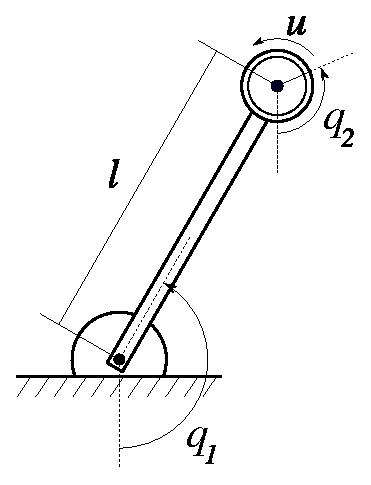
\includegraphics[width=0.25\linewidth]{figures/iwp.eps}
    \caption{Schematic of the inertia wheel pendulum. Only the joint $q_2$ is actuated, and $q_1$ is not.}
    \label{fig:iwp}
\end{figure}

\subsubsection{Training} 

The energy-like function $H_d^\theta$ is a fully-connected neural network with
two hidden layers, each with the \textsc{Elu} activation
function~\cite{clevert2015fast}. 
%
% There are, in total, 137 parameters to learn. 
% %
% They are initialized according to the Glorot
% (Xavier)~\cite{glorot2010understanding} scheme.
%
% The objective of the optimization problem~\eqref{eq:neural_pbc_finite_optim}
% consists of $\ell_{\textrm{set}}$ given by Equation~\eqref{eq:set_distance},
% with the set $\mathcal{S}$ chosen as a ball of radius $r = 0.01$ around
% $x^\star$ in the standard norm topology.
%
A uniform distribution in $[-2\pi, 2\pi] \times [-2\pi, 2\pi] \times [-10, 10]
\times [-10, 10]$ is chosen as the probability distribution from which samples
of initial states $x_0$ are drawn for the \textsc{DAgger} strategy.
%
In each gradient descent step, we sample a batch of 4 initial states
$\{x_0\}$ from $x_0 \sim \mathcal{N}(x^\star, \Sigma_0)$ and \textsc{DAgger}
as discussed in Section~\ref{ssec:state_sampling}; these initial states are
integrated forward with a time horizon of $t \in [0,3]$ seconds. 
%
In the Bayesian framework, the standard deviations $\sigma_{\zeta}$ of system
parameters $\zeta = [I_1, I_2, mgl]$ are chosen to be $10\%$ of the nominal system
parameters given in Section~\ref{sec:iwp}.
%
Moreover, we train on trajectories per the SDE
in~\eqref{eq:neural_bayesian_inference} with measurement error represented
by Wiener process with standard deviation of 0.001 and 0.02 on the joint
angles and velocities, respectively.
%
% In each gradient descent step, a batch of 4 initial conditions $\{x_0\}$
% generated by \textsc{DAgger} is integrated forward with using the Tsitouras
% $5(4)$ Runge-Kutta solver with a time horizon of $t \in [0,3]$ seconds. 
%
% The cost function is then computed and back-propagated using the
% AD-assisted adjoint method implemented in
% \verb|DiffEqFlux.jl|~\cite{DBLP:journals/corr/abs-2001-04385}.
% %
% In the Bayesian learning framework, we draw samples from the posterior and
% back-propagate through the gradients of the \textsc{Elbo} using the
% \textsc{ADVI}~\cite{kucukelbir2015automatic} scheme provided in
% \verb|Turing.jl|~\cite{turing}. 
%

We use variational inference to estimate a Gaussian posterior distribution
over uncorrelated parameters. The trainings are terminated when the loss
function $J(\gamma) = J_{set}(\gamma) + J_T(\gamma)$ and the \textsc{Elbo}
converge for the deterministic and Bayesian trainings, respectively.
%
The hyperparameters for the deterministic and Bayesian \textsc{NeuralPbc}
trainings are shown in Table~\ref{tab:training_setup_neuralpbc}.
%
It can be seen that the Bayesian training effectively learns with smaller
neural network size than the deterministic training.
\begin{table}[tb]
    \centering
    \caption{\textsc{NeuralPBC} training setup for deterministic and Bayesian frameworks}
    % \rowcolors{2}{}{Wheat1}
    \begin{tabular}{lcc}
    \toprule
    %   & \multicolumn{2}{c}{Framework} \\
    %   \cmidrule(lr){2-3}
    & Deterministic & Bayesian \\
    \midrule
        $H_d$ neural net size & (6, 12, 3, 1) & (6, 5, 3, 1)\\
        Learned parameters & 133 & 128  \\
        Optimizer & \textsc{ADAM} & DecayedAdaGrad\\
        Initial learning rate & 0.001 & 0.01\\
        Replay buffer size & 400 & 50\\
    \bottomrule
    \end{tabular}
    \label{tab:training_setup_neuralpbc}
\end{table}

\subsubsection{Simulation Tests} 
The performance of the controllers obtained from the deterministic and Bayesian
trainings are compared as follows.
%
We evaluate the performance of both trainings with parameter uncertainties
on $I_1, I_2$ and $mgl$. 
%
We introduce these uncertainties by moving the average
system parameters by $\pm 10\%$ to $\pm 50\%$ with increments of $10\%$. 
%
For each average system parameter, we sample uniformly with a $\pm 5\%$ support
around the average system parameters. 
%
This helps test the performance of the controller with various combinations of
$I_1, I_2$ and $mgl$.
%
On top of the system parameter uncertainties, we introduce measurement noise
represented by a Wiener process with standard deviation of $0.001$ and $0.02$ on
the joint angles and velocities, respectively. 
%
Figure~\ref{fig:comparison_neuralpbc} shows the performance of deterministic and
Bayesian trainings using an accumulated quadratic loss of the form
\begin{equation} J^T = \frac{1}{2}\int_0^T \left(x^\top Qx + u^\top Ru \right) dt.
\label{eq:performance_metric} \end{equation}
%
The controller learned from the Bayesian training is marginalized over 10
parameters sampled from the posterior.
As seen in Figure~\ref{fig:comparison_neuralpbc}, the Bayesian training
effectively collects less cost for large error in system parameters.
%
Moreover, the error band on the cost of the Bayesian training is smaller than
that of the deterministic training; this shows that the marginalized controller
is more robust against measurement noise.
%   
\begin{figure}
    \centering
    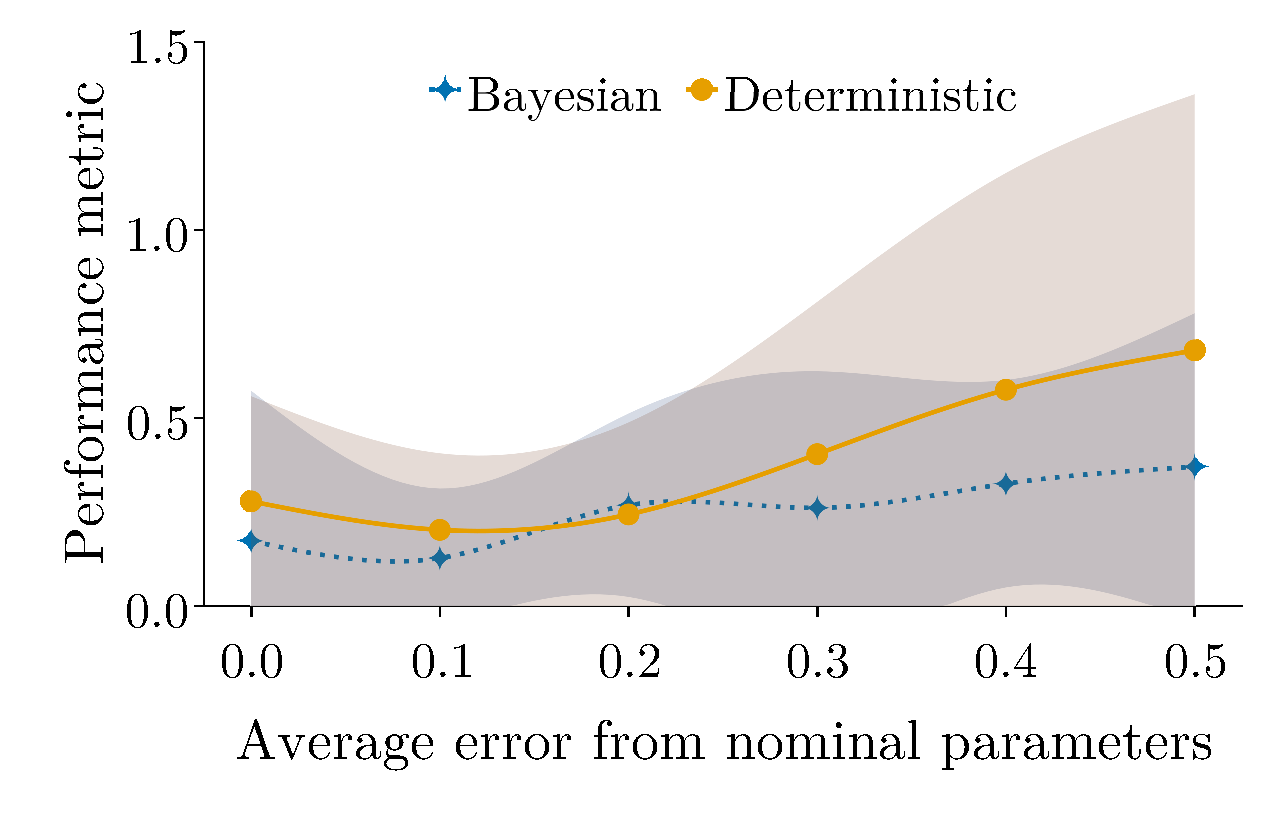
\includegraphics[clip,width=0.7\linewidth]{./figures/bandplot2.eps}%
    \caption{\textsc{NeuralPBC} Performance metric ($J^T$) for various
    error in system parameters. Measurement noise included as Wiener process
    with standard deviation of $0.001$ and $0.02$ on joint angles and
    velocities, respectively}
    \label{fig:comparison_neuralpbc}
\end{figure}

\subsubsection{Hardware Tests} 
The controllers from deterministic and Bayesian training schemes are
evaluated on hardware. 
%
We deliberately modify the hardware and test the controllers without any
additional training.
%
In particular, throughout the experiments, the inertia wheel attached to $q_2$
is replaced with parts (labelled A-C on Table~\ref{tab:modified_params}) whose
mass and inertia are different from the nominal values.
%
The modified system parameters are summarized in
Table~\ref{tab:modified_params}.
%
% The parameter error listed on the last column of Table~\ref{tab:modified_params}
% is computed by $\|p - p_{\textrm{nom}}\| / \|p_{\textrm{nom}}\|$.
\begin{table}[tb]
    \centering
    \caption{System parameters used in real-world experiments. The errors in the
    last column are $\|p_s - p^{\textrm{nom}}_{s}\| / \|p^{\textrm{nom}}_{s}\|$}.
    % \rowcolors{2}{}{Wheat1}
    \begin{tabular}{lcccc}
    \toprule
    Parameter set $p_s$ & $I_1$ & $I_2$ & $mgl$ & Error \\
    \midrule
    Nominal & 0.0455 & 0.00425 & 1.795 & 0 \\
    A & 0.0417 & 0.00330 & 1.577 & $0.122$ \\
    B & 0.0378 & 0.00235 & 1.358 & $0.243$ \\
    C & 0.0340 & 0.00141 & 1.140 & $0.365$ \\
    \bottomrule
    \end{tabular}
    \label{tab:modified_params}
\end{table}
    
The system starts from rest at the downward position. 
%
A small disturbance in the $q_1$ direction is introduced to start the swing-up.
%
The state $x$ is recorded and~\eqref{eq:performance_metric} is the
performance metric used to evaluate the controllers. The results are
summarized in Figure~\ref{fig:neuralpbc_bar_plot}.
%
\begin{figure}[t]
    \centering
    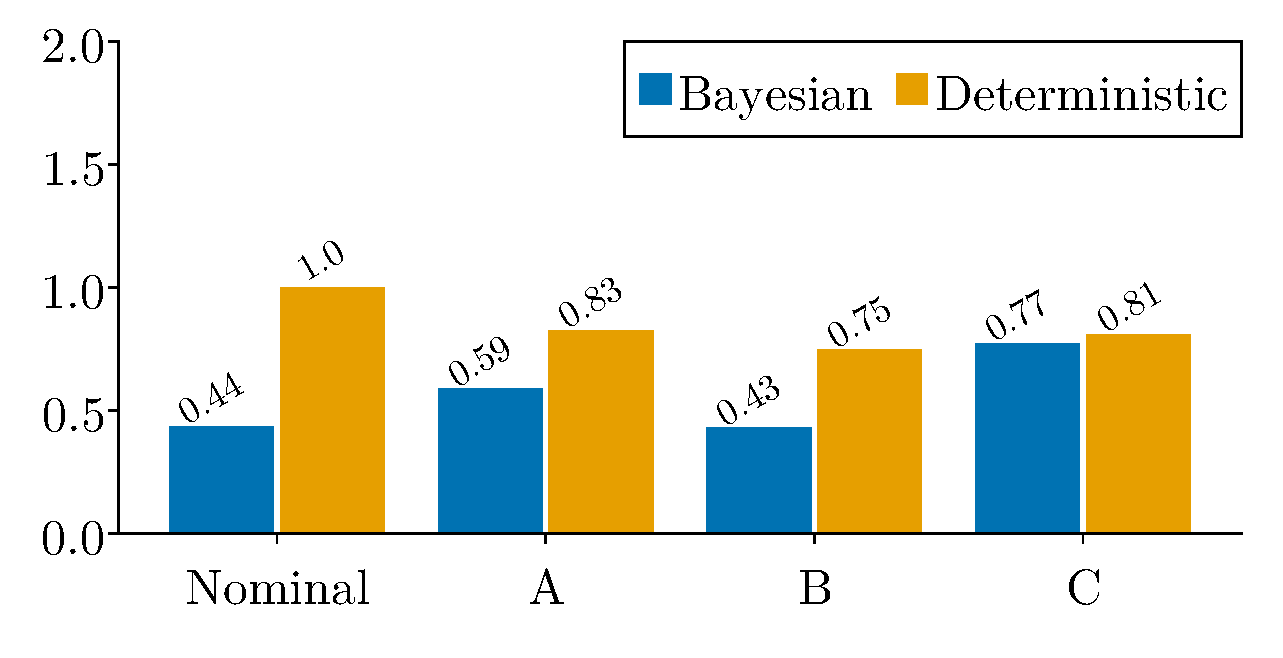
\includegraphics[width=0.6\linewidth]{./figures/pbc_bar.eps}
    \caption{
        %
        Controller performance for modified system parameters. 
        %
        The performance metric is given by
        Eq.~\eqref{eq:performance_metric}.
        %
        Lower values are better. 
        %
        These results show that controllers trained via Bayesian learning are
        consistently more robust to errors in system parameters.
        %
    }
    \label{fig:neuralpbc_bar_plot}
\end{figure}

In all scenarios, our controllers are able to achieve the control objective
despite the errors introduced in the system parameters.
%
% Furthermore, the controller from Bayesian training consistently outperforms the
% controller from deterministic training, supporting the theoretical justification
% discussed in Section~\ref{ssec:justification}. 
%
These results demonstrate that our approach enables a unified way to tackle
nonlinear control problems while simultaneously incorporating prior knowledge
and model uncertainties.
%
  
%%%%%%%%%%%%%%%%%%%%%%%%%%%%%%%%%%%%%%%%%%%%%%%%%%%%%%%%%%%%%%%%%%%%%%%%%%%%%%%%%%%
%%%%%%%%%%%%%%%%%%%%%%%%%%%%%%%%%%%%%%%%%%%%%%%%%%%%%%%%%%%%%%%%%%%%%%%%%%%%%%%%%%%

\subsection{Control Design for Hybrid Dynamical Systems}
\label{ssec:pbc_hybrid}

In this section, we extend the techniques of deterministic and Bayesian \textsc{NeuralPbc} to hybrid dynamical systems.
%
We introduce an accurate model of the hybrid dynamics into the deterministic \textsc{NeuralPbc} framework and infer a controller that either leverages the advantages of contact events and minimizes its adverse effects.
%
Moreover, we inject uncertainties in contact forces and post-impact velocities to \textsc{NeuralPbc} in order to design a robust controller through Bayesian learning.
%




\subsubsection{Deterministic \textsc{NeuralPbc}}
\label{sssec:data_driven_neuralpbc}

In this framework, we aim to find a passive closed loop system for the hybrid
dynamics~\eqref{eq:hybrid_dynamics} whose desired stable equilibrium is at
$(q^*, \dot{q}^*)$.
%
We formulate this problem as a search over the point-estimate parameters of
$H_d$ given by a neural network.
%
This training framework can be posed as the following optimization problem. 
\begin{equation}
    \begin{aligned}
        \underset{\theta}{\textrm{minimize}} 
        & & &\int_{0}^{T} \ell \left(\phi,u^{\theta}(\phi) \right) \, \dd t , \\%
        \textrm{subject to}
        & & M(q) &\dd \dot{q} + h(q, \dot{q}, \theta)\dd t - \dd R  = 0,\\%
        & & u^{\theta} &= -\Omega^{\dagger} (\nabla_q H_d^{\theta} - \nabla_q H),%
    \end{aligned}
    \label{eq:hybrid_neuralpbc}
\end{equation}
%
The performance objective $\ell$ is evaluated from closed loop trajectories
generated from various initial states.
%
We follow Moreau's time stepping algorithm~\cite{glocker2005formulation} outline
in Algorithm~\eqref{algo:moreau} to resolve the complementarity constraint
in~\eqref{eq:complementarity} and numerically integrate the measure differential
equations~\eqref{eq:dynamics}.
%

We intend to find a solution to the optimization problem
in~\eqref{eq:hybrid_dynamics} for all initial states $(q_0, \dot{q}_0)$ in the
state space.
%
To efficiently sample the initial states, we use a combination of greedy and
explorative state sampling techniques.
%
The greedy state sampling, commonly known as \textsc{DAgger}~\cite{ross2011no},
generates trajectories using the current $H_d$ parameters and collects $N_d$
samples from the visited states. 
%
This allows the training to refine the controller on the states it visits the
most.
%
We recover from locally optimal solutions through explorative state sampling,
which takes $N_r$ number of random samples from the state space.
%
In a single batch training, we compute the performance objective as an expectation
over $N_{\mathcal{D}} = N_d+N_r$ samples as follows:
\begin{align*}
    J(\theta) = \mathbb{E}_{q_0, \dot{q}_0 \sim \mathcal{D}_N}[ \ell(\phi(t; q_0, \dot{q}_0), u^\theta)]
\end{align*}
\noindent where $\mathcal{D}_N$ is a collection of $N_{\mathcal{D}}$ initial state samples.


As outlined in Algorithm~\ref{algo:deter_neuralpbc}, we compose the cost
$\ell$ from the $N_{\mathcal{D}}$ closed loop trajectories and update the
parameters $\theta$ through stochastic gradient descent (SGD). 
%
We compute the gradient $\nicefrac{\partial \ell}{\partial \theta}$ through
auto-differentiation techniques.
%

\begin{algorithm}
  \setstretch{1.2}
    \caption{Solution to the Optimization Problem~\eqref{eq:hybrid_neuralpbc}}
    \label{algo:deter_neuralpbc}
    \small
    \begin{algorithmic}[1]
        \algrenewcommand\algorithmicindent{0em} % No indent
        \State $\mathcal{D}_N \gets \{q_0, \dot{q}_0\}_{(N_{\mathcal{D}})}$  \Comment{$N_{\mathcal{D}}$ initial state samples} 
        \algrenewcommand\algorithmicindent{1.1em} % Change indent back to default
        \While{$i < $ \texttt{maximum iteration}}
        \State $J \gets 0$\Comment{Batch loss}
        \For{$(q_0, \dot{q}_0) \sim \mathcal {D}_N$}
            \State $\phi$ = Moreau($q_0, \dot{q}_0$) \Comment Algorithm~\eqref{algo:moreau}
            \State $J \gets J + \ell(\phi; \theta)/N_{\mathcal{D}}$ \Comment{Batch loss}
        \EndFor
        \State $\theta \gets \theta + \alpha_i \nicefrac{\partial J}{\partial \theta}$\Comment{SGD step}
        \State $\mathcal{D}_N \gets \{q_0, \dot{q}_0\}_{(N_{\mathcal{D}})}$\Comment{New initial state samples}
        \State $i \;\:\gets i + 1$
        \EndWhile
        \State \textbf{return} $\theta$
    \end{algorithmic}
\end{algorithm}

\subsubsection{Bayesian \textsc{NeuralPbc}}
\label{sssec:bayesian_inference}

Walking machines such as the rimless wheel are bound to experience undetermined
external forces from uneven terrain.
%
If the robot does not respond to these external disturbances in real-time, they
can cause underperformance or even instability.
%
In order to learn a controller robust against these uncertainties, we inject
domain randomization on the state of the environment during the training
process.
%
Unfortunately, simply introducing random environmental conditions to the
training outlined in Algorithm~\ref{algo:deter_neuralpbc} is not sufficient. 
%
In the presence of high variance disturbances, the point-estimate parameters
$\theta$ under domain randomization are prone to be
biased~\cite{ashenafi2022robustness};
%
for instance, if the uncertainty in the terrain elevation is large, the learned
parameters $\theta$ may be far from the optimal controller corresponding to
the true elevation.
%
To combat this issue, we propose a probabilistic framework, where we learn a
posterior probability distribution over the parameters $\theta$ via Bayesian
inference. 
%
Then we address the bias-variance trade-off problem by marginalizing the
controller over the distribution of the parameters~\cite{bishop2006pattern}.

In the probabilistic framework, we parameterize the desired Hamiltonian $H_d$
with a Bayesian neural network, whose weights and biases are samples drawn from
a posterior probability distribution~\cite{jospin2020hands}.
%
The objective is to find the posterior distribution $P(\theta |J)$ that achieves
the performance objective for various environmental conditions.
%
This framework can be summarized by the following optimization problem.

\begin{equation}
    \begin{aligned}
        \underset{P(\theta)}{\textrm{minimize}} 
        & & &\int_{0}^{T} \ell \left(\phi,u^{\theta}(\phi) \right) \, \dd t , \\
        \textrm{subject to}
        & & M(q) &\dd \dot{q} + h(q, \dot{q}, \theta)\dd t - \dd R  = 0,\\
        & & u^{\theta} &= -\Omega^{\dagger} (\nabla_q H_d^{\theta} - \nabla_q H), \\
        & & p_s &\sim \mathcal{U}(p_{min}, p_{max}), \\
        & & \theta &\sim P(\theta).
    \end{aligned}
    \label{eq:bayesian_hybrid_neuralpbc}
\end{equation}
\noindent The random variable $p_s \in \mathbb{R}^{N}$ is sampled from $N$
uncorrelated uniform probability distributions $\mathcal{U} \sim [p_{min}, p_{max}]$
with lower bound $p_{min}$ and upper bound $p_{max}$.
%
The magnitude of the samples $p_s$ determine the elevation of the terrain under
each spoke, which consequently randomize the gap $g_N$, pre-impact velocities
$\dot{q}^{-}$ and contact forces between each spoke and the ground.

From Bayes' theorem, the posterior distribution $P(\theta |J)$ is a function of
the prior distribution $P(\theta)$ and the likelihood function $P(J |
\theta)$~\cite{bishop2006pattern}.
\begin{align}
  P(\theta | J) = \frac{P(J | \theta) P(\theta)}{\int P(J | \theta) P(\theta) \; d \theta}
  \label{eq:bayes}
\end{align} 
The prior can be used to inject any former knowledge about the controller. 
%
For instance, an informed prior can be a normal distribution whose mean is the
solution to the optimization problem in~\eqref{eq:hybrid_neuralpbc}. If there is
no prior information, $P(\theta)$ can be set as a uniform distribution.
%
The likelihood function consists of the expected performance $J$ in the following form:
\begin{align}
  P(J|\theta) = \mathcal{N}(0, s),
  \label{eq:likelihood}
\end{align}
\noindent where $s$ is the standard deviation of the likelihood.
%


There are various techniques to find the exact posterior
distribution~\cite{bishop2006pattern}, but they have weak scalability
for high-dimensional systems. Thus, we use variational inference, a technique
that approximates the posterior with the distribution $Q(\theta;z)$ selected
from the conjugate family of the prior~\cite{cohen2016bayesian}. 
%
The goal is to learn the distribution parameters $z$ of the chosen posterior.
%
The performance objective that minimizes the loss $J$ while also matching the 
approximate posterior $Q$ to the exact one is
\begin{align}
  \mathcal{L}(J, z) = \mathbb{E}_{\theta \sim Q}[ \log{(P(J | \theta) P(\theta))} - \log{(Q(\theta;z))}]
  \label{eq:elbo}
\end{align}
\noindent where $\mathcal{L}(J, z)$ is the evidence lower bound (\textsc{Elbo})~\cite{tipping2003bayesian}.
%

As outline in Algorithm~\eqref{algo:bayes_neuralpbc}, we update the distribution
parameters of the posterior $Q(\theta;z)$ through stochastic gradient descent. 
%
We use auto-differentiation techniques to take the gradient of the \textsc{Elbo}
with respect to $z$.
%
We invoke the reparameterization trick of the Automatic Differentiation
Variational Inference (ADVI)~\cite{kucukelbir2015automatic} to compute the
gradient of~\eqref{eq:elbo} through the samples drawn from the posterior.

\begin{algorithm}
  \setstretch{1.2}
    \caption{Solution to the Optimization Problem~\eqref{eq:bayesian_hybrid_neuralpbc}}
    \label{algo:bayes_neuralpbc}
    \small
    \begin{algorithmic}[1]
        \algrenewcommand\algorithmicindent{0em} % No indent
        \State $\mathcal{D}_N \gets \{q_0, \dot{q}_0\}_{(N_{\mathcal{D}})}$  \Comment{$N_{\mathcal{D}}$ initial state samples} 
        \algrenewcommand\algorithmicindent{1.1em} % Change indent back to default
        \While{$i < $ \texttt{maximum iteration}}
        \State $\mathcal{L} \gets 0$ \Comment{\textsc{Elbo} Loss}
        \For{$i=1:Q_N$} \Comment{Samples to compute~\eqref{eq:elbo}}
        \State $J \gets 0$ \Comment{Batch loss}
        \State $\theta \sim Q(\theta; z)$ \Comment{Sample parameters of $H^\theta_d$}
          \For{$(q_0, \dot{q}_0) \sim \mathcal {D}_N$}
            \State $p_s \sim \mathcal{U}(p_{min}, p_{max})$
            \State $\phi$ = Moreau($q_0, \dot{q}_0$) \Comment Algorithm~\eqref{algo:moreau}
            \State $J \gets J + \ell(\phi; \theta)/N_{\mathcal{D}}$ 
          \EndFor
        \State $\mathcal{L} \gets \mathcal{L} + \frac{1}{Q_N} \left(\log[P(J | \theta) P(\theta)] - \log[Q(\theta;z)]\right)$
        \EndFor
        \State $z \gets z + \alpha_i \nicefrac{\partial \mathcal{L}}{\partial z}$\Comment{SGD step}
        \State $\mathcal{D}_N \gets \{q_0, \dot{q}_0\}_{(N_{\mathcal{D}})}$\Comment{New initial state samples}
        \State $i \;\:\gets i + 1$
        \EndWhile
        \State \textbf{return} $z$
    \end{algorithmic}
\end{algorithm}


\subsection{Rimless Wheel}
\label{sssec:rimless_wheel_model}

This mechanism consists of a rimless wheel in the plane with a set of $N$ spokes
and a torso freely rotating about a pin joint located at the center of the
wheel.
% 
The mass of the wheel $m_1$ is concentrated at the hip and spans a radius of
$l_1$.
%
The torso has its mass $m_2$ concentrated at a distance of $l_2$ from the hip. 
%
We actuate the torso angle with the motor mounted at the hip, which in turn
propels the entire wheel. 
%
The angle of the torso is characterized by $\varphi$ measured from the outward
normal of the runway shown as $\hat{n}$ in Figure~\ref{fig:rimless_wheel_w_torso}.  
%
The orientation of the wheel $\beta$ is measured from $\hat{n}$ to a datum spoke.
%

\begin{figure}[b]
 \centering
 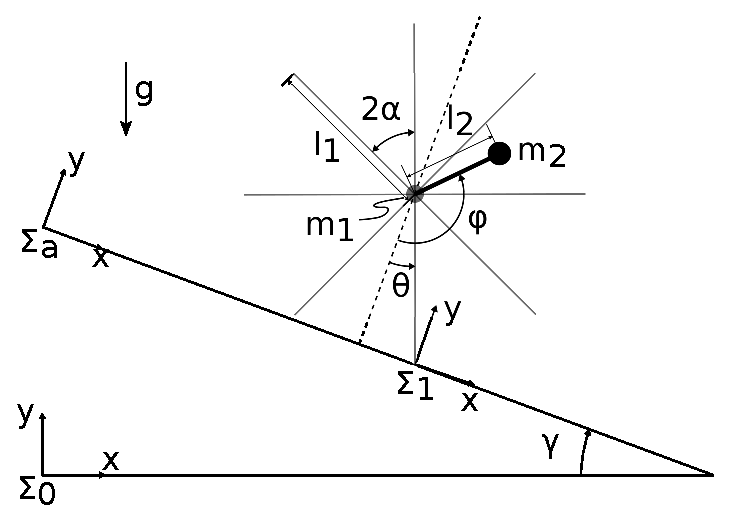
\includegraphics[width=0.75\columnwidth]{./figures/rimless_wheel_with_torso_v3.eps}
 \caption{Rimless wheel with torso depicted with $N=10$ spokes.}
 \label{fig:rimless_wheel_w_torso}
\end{figure}

% \subsubsection{Equations of motion}
Rimless wheel is a system that undergoes phases of continuous flows and discrete
transitions, resulting in a hybrid dynamical system with two modes. We construct
a dynamical model for such system with the Lagrangian approach. The kinetic and
potential energies of the system are given by

\begin{equation*}
  \begin{gathered}
    \mathcal{K} = \frac{1}{2} m_t(\dot{x} + \dot{y})^2  +  \frac{1}{2} I_1 \dot{\beta}^2  + 
                    \frac{1}{2} (m_2 l_2^2 + I_2) \dot{\varphi}^2 + m_2 l_2(c_{\varphi} \dot{x} + s_{\varphi} \dot{y}) \dot{\varphi} \\
    \mathcal{P} = m_tg(-x s_{\gamma} + y c_\gamma) - m_2 g l_2 c_{\varphi \gamma}
  \end{gathered}
\end{equation*}

\noindent where $c_a := \cos{(a)}, s_a := \sin{(a)}, c_{ab} := \cos{(a - b)},
s_{ab} := \sin{(a - b)}$. The total mass of the mechanism is given by $m_t$;
$I_1$ and $I_2$ are moments of inertia of the wheel and torso respectively. The
position vector $(x, y)$ represents the location of the hip with respect to the
frame $\Sigma_1$ shown in Figure~\ref{fig:rimless_wheel_w_torso}. The slope of
the runway is given by $\gamma$, $g$ is the magnitude of acceleration due to
gravity.
%
The Euler-Lagrange equations corresponding to the Lagrangian $\mathcal{L} =
\mathcal{K} - \mathcal{P}$ are

\begin{equation}
  M(q) \dd \dot{q} + h(q, \dot{q})\dd t - \dd R  = 0,
  \label{eq:dynamics}
\end{equation}

\begin{equation*}
  \begin{gathered}
    h(q, \dot{q}) = C(q, \dot{q})\dot{q} + G(q) - Bu(q, \dot{q}),\\
    M(q) = \bmat{m_t & 0 & m_2 l_2 c_{\varphi} & 0 \\ 0 & m_t & m_2 l_2 s_{\varphi} & 0 \\
            m_2 l_2 c_{\varphi} & m_2 l_2 s_{\varphi} & I_2+m_2 l_2^2 & 0 \\
            0 & 0 & 0 & I_1}, \\
    C(q,\dot{q}) = m_2l_2 \bmat{0 & 0 & -s_{\varphi} \dot{\varphi} & 0\\ 
                    0 & 0 & c_{\varphi} \dot{\varphi} & 0 \\ 
                    -s_{\varphi} \dot{\varphi} & c_{\varphi} \dot{\varphi} & 0 & 0 \\
                    0 & 0 & 0 & 0}, \\
    G(q) = g\bmat{-m_t s_{\gamma} & 
                  m_t c_{\gamma} &
                  m_2 l_2 s_{\phi,\gamma} &
                  0}^\top \\
  \end{gathered}
\end{equation*}

\noindent where $q = (x, y, \varphi, \beta)$, $B = \bmat{0 & 0 & 1 & -1}^\top$,
$u(q, \dot{q})$ is the torque applied to the torso and $\dd R$ represents the
force measure of contact forces and Coulomb friction exerted on the spokes by
the ground. We use the linear complementarity
formulation~\cite{glocker2005formulation} to resolve the contact forces and
Coulomb friction contributing to the discrete transitions.


\subsubsection{Training}
\label{sssec:training}

Both the deterministic and Bayesian frameworks learn $H_d$ given by a
fully-connected neural network with a total of 113 weights and biases.   
%
A single parameter update consists of a batch of 4 initial states sampled
through greedy or explorative techniques.
%
Each initial state is integrated forward for time horizon of 5 seconds.
%
The objective of the trainings is to use the control authority on the torso to
move the robot at a constant hip speed.
%
The performance objective is given by the accumulated loss
\begin{align}
    J_T = \int_0^{T} \ell(\phi(t); \theta) \dd t = \sum_{t=0}^{T} (\dot{x}^* - \dot{x}(t; \theta))
    \label{eq:loss}
\end{align}
\noindent where $\dot{x}^*$ is a constant 1 \nicefrac{m}{s}.
%
For the Bayesian training, we generate random terrain elevation parameters $p_s$
from a uniform probability distribution $\mathcal{U} \sim[0, 3]$ centimeters.


\subsubsection{Simulated Experiments}

We first show the performance of the deterministic \textsc{NeuralPbc} training
on a level ground.
%
As shown on the bottom plot of Figure~\ref{fig:deter_rw_trajectory}, the robot
starts from rest and slowly reaches the desired hip speed.
%
The top plot shows that the controller learned to apply large torque
when the wheel is at rest and then the torso maintains a constant angle, which
is sufficient to create constant hip speed on level ground.  
%
During discrete transitions (shown with dashed-red lines), the angular velocity
of the torso counteracts the forward motion of the wheel, but a large torque is
applied quickly to maintain the torso angle.
%
The torque plot on Figure~\ref{fig:deter_control} shows that a large
positive torque is applied if the wheel stumbles backwards.
%

\begin{figure}[H]
    \centering
    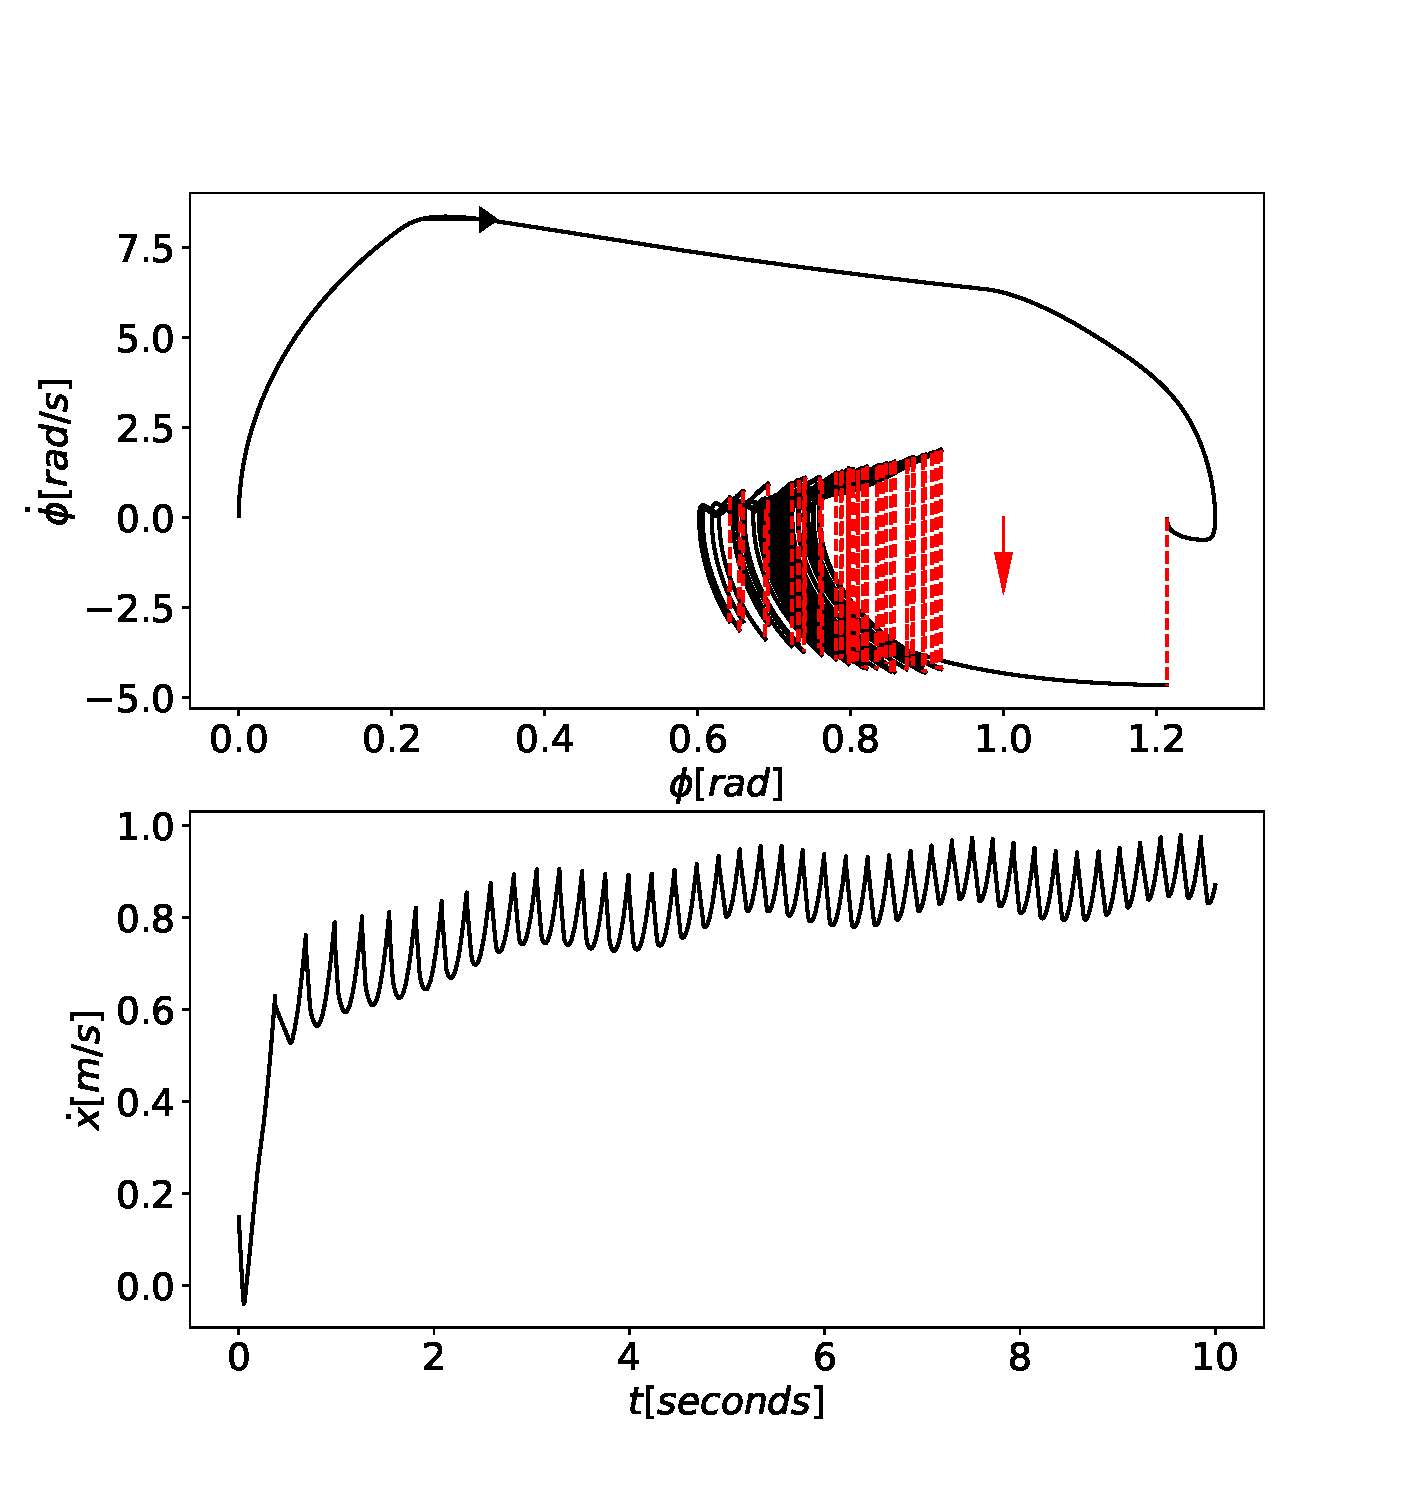
\includegraphics[width=0.8\columnwidth]{RW_deter_trajectory.eps}
    \caption{Top: Torso orientation and velocity for 10-second trajectory. The
            solid black lines show the continuous phases and the dashed red
            lines show discrete transitions. Bottom: Horizontal hip speed}
    \label{fig:deter_rw_trajectory}
\end{figure}

\begin{figure}[H]
    \centering
    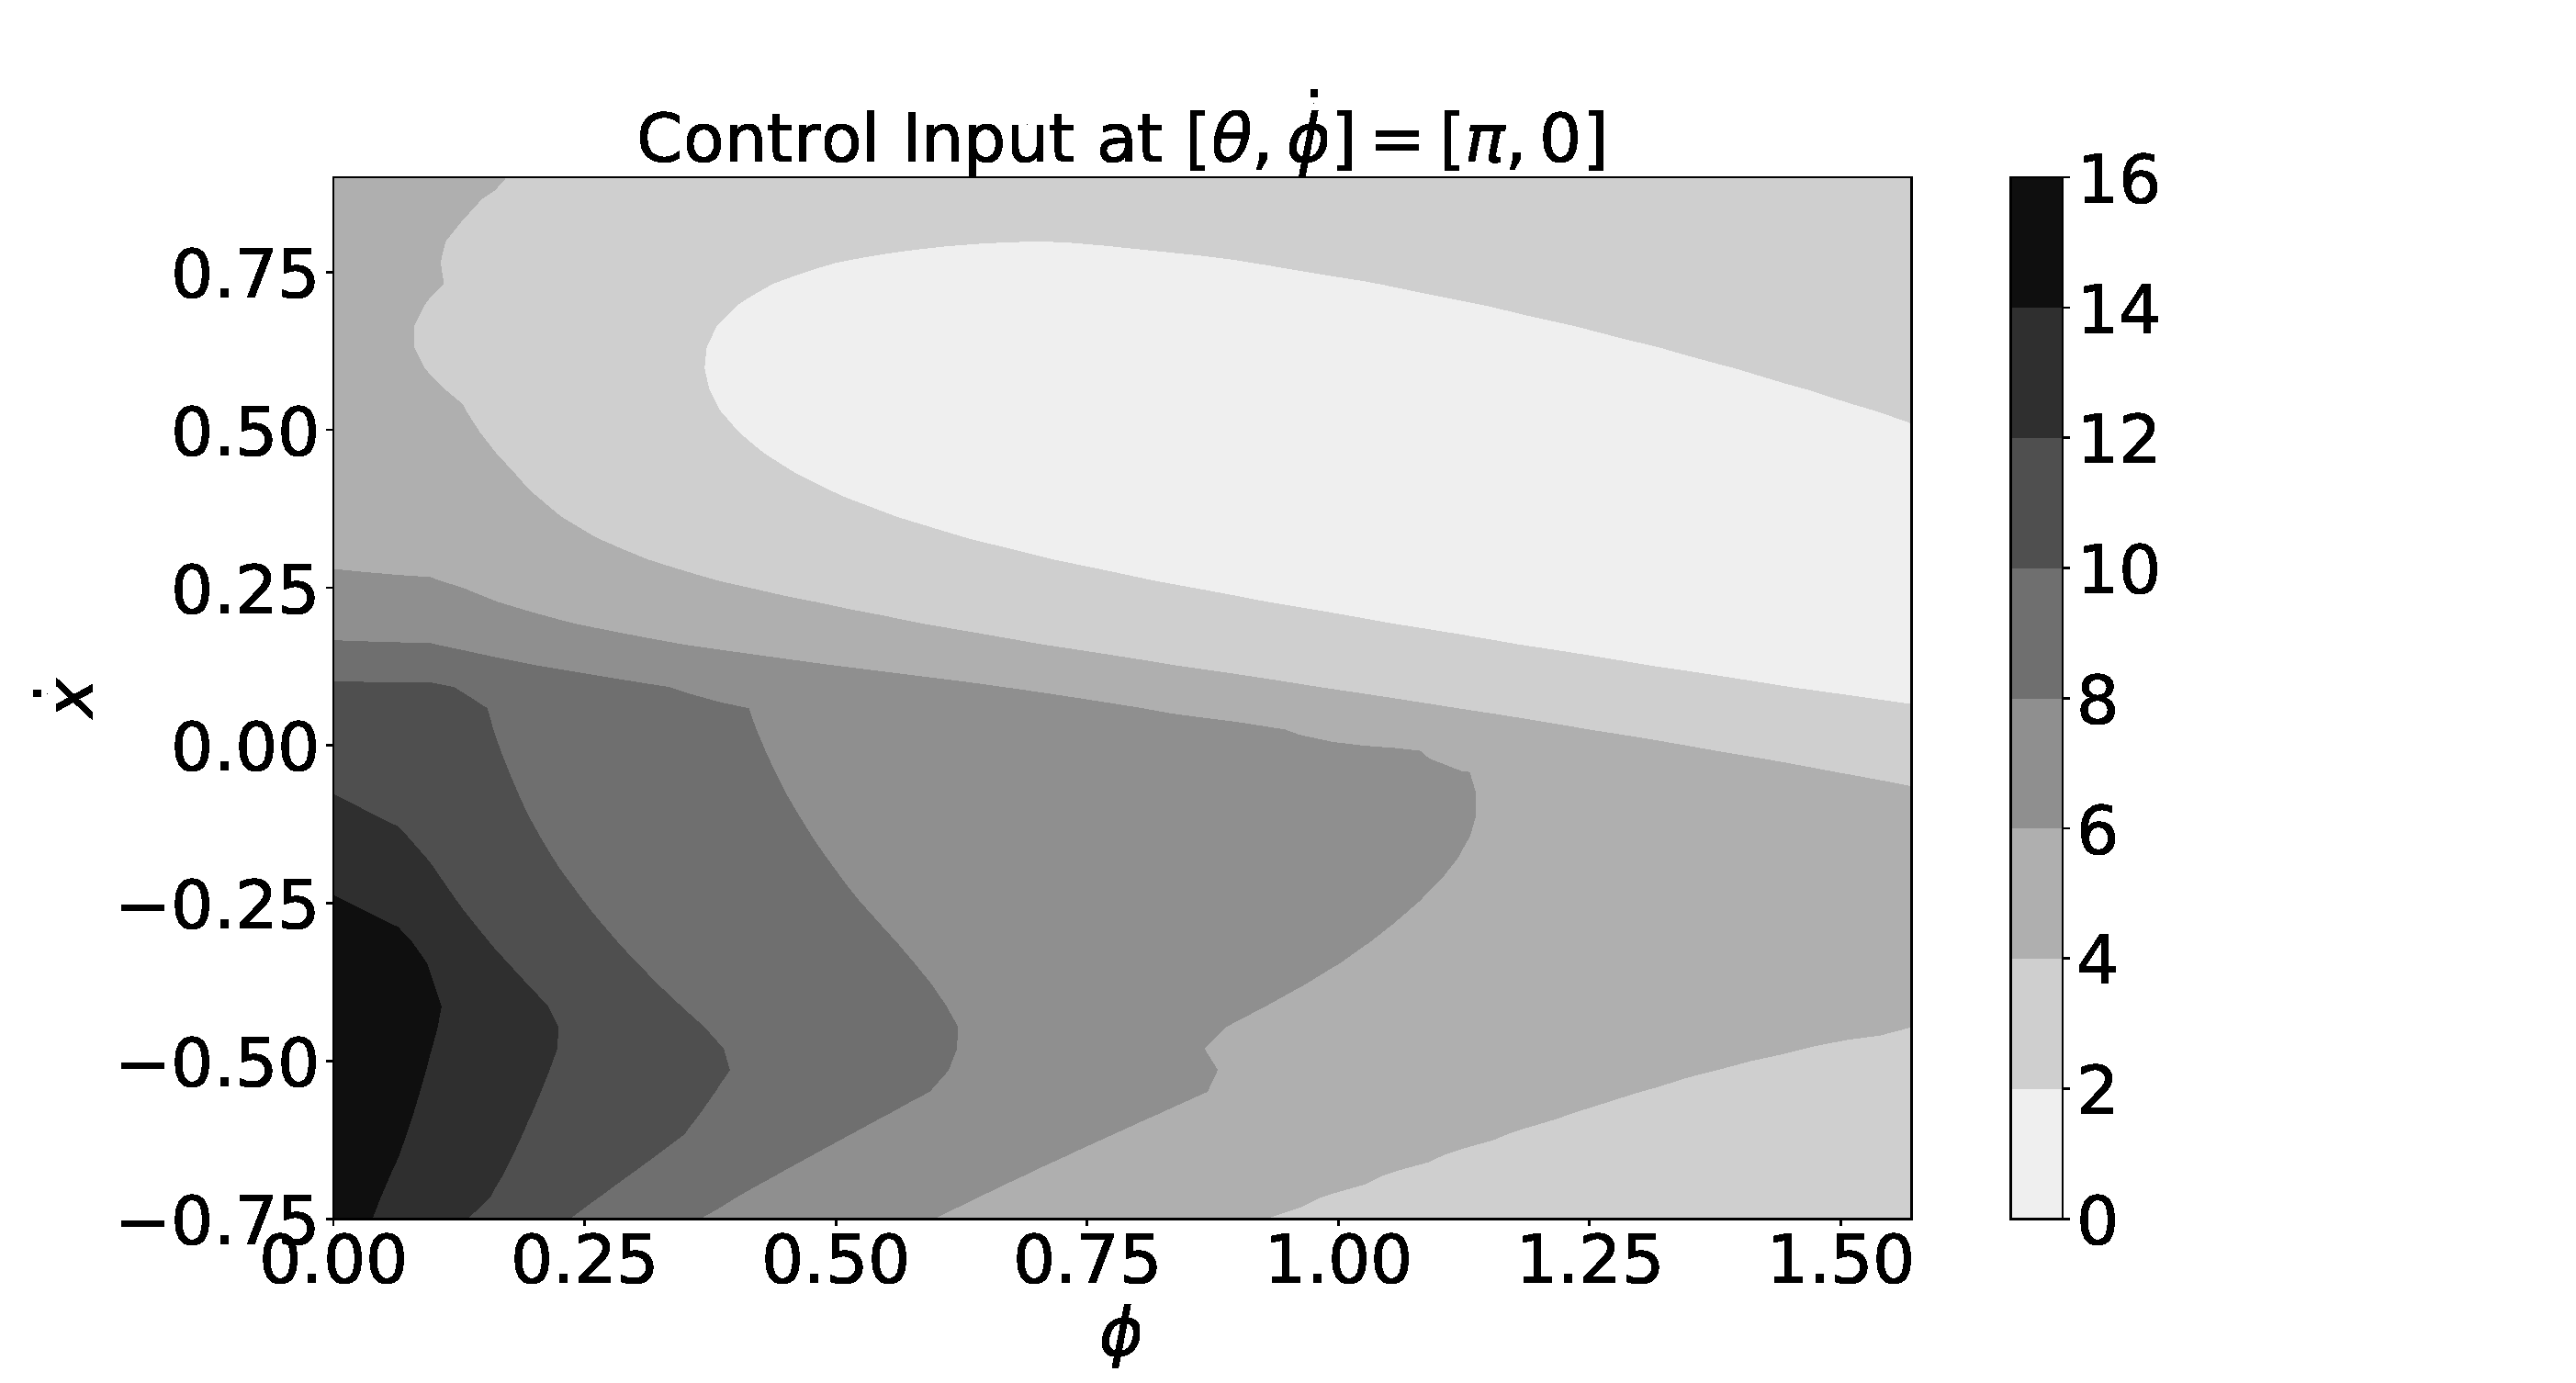
\includegraphics[width=0.9\columnwidth]{RW_deterministic_control.eps}
    \caption{Torque command to torso as a function of torso angle and horizontal hip speed}
    \label{fig:deter_control}
\end{figure}
We compare the performance of the two controllers as follows.
%
Similar to the Bayesian training, we sample the terrain elevation from
$\mathcal{U} \sim[0, p_{max}]$ where $p_{max} = [0, 0.5, 1, 1.5, 2]$ centimeters.
%
For each value of $p_{max}$, we generate 10 random initial states $(q_0,
\dot{q}_0)$ and integrate 10-second trajectories.
%
The cost of each trajectory is calculated as per~\eqref{eq:loss}.
%
The solid line in Figure~\ref{fig:comparison} shows the average $J_T$ over the
10 trajectories for each $p_{max}$ and the error band represents the standard
deviation over the accumulated losses.

\begin{figure}[H]
    \centering
    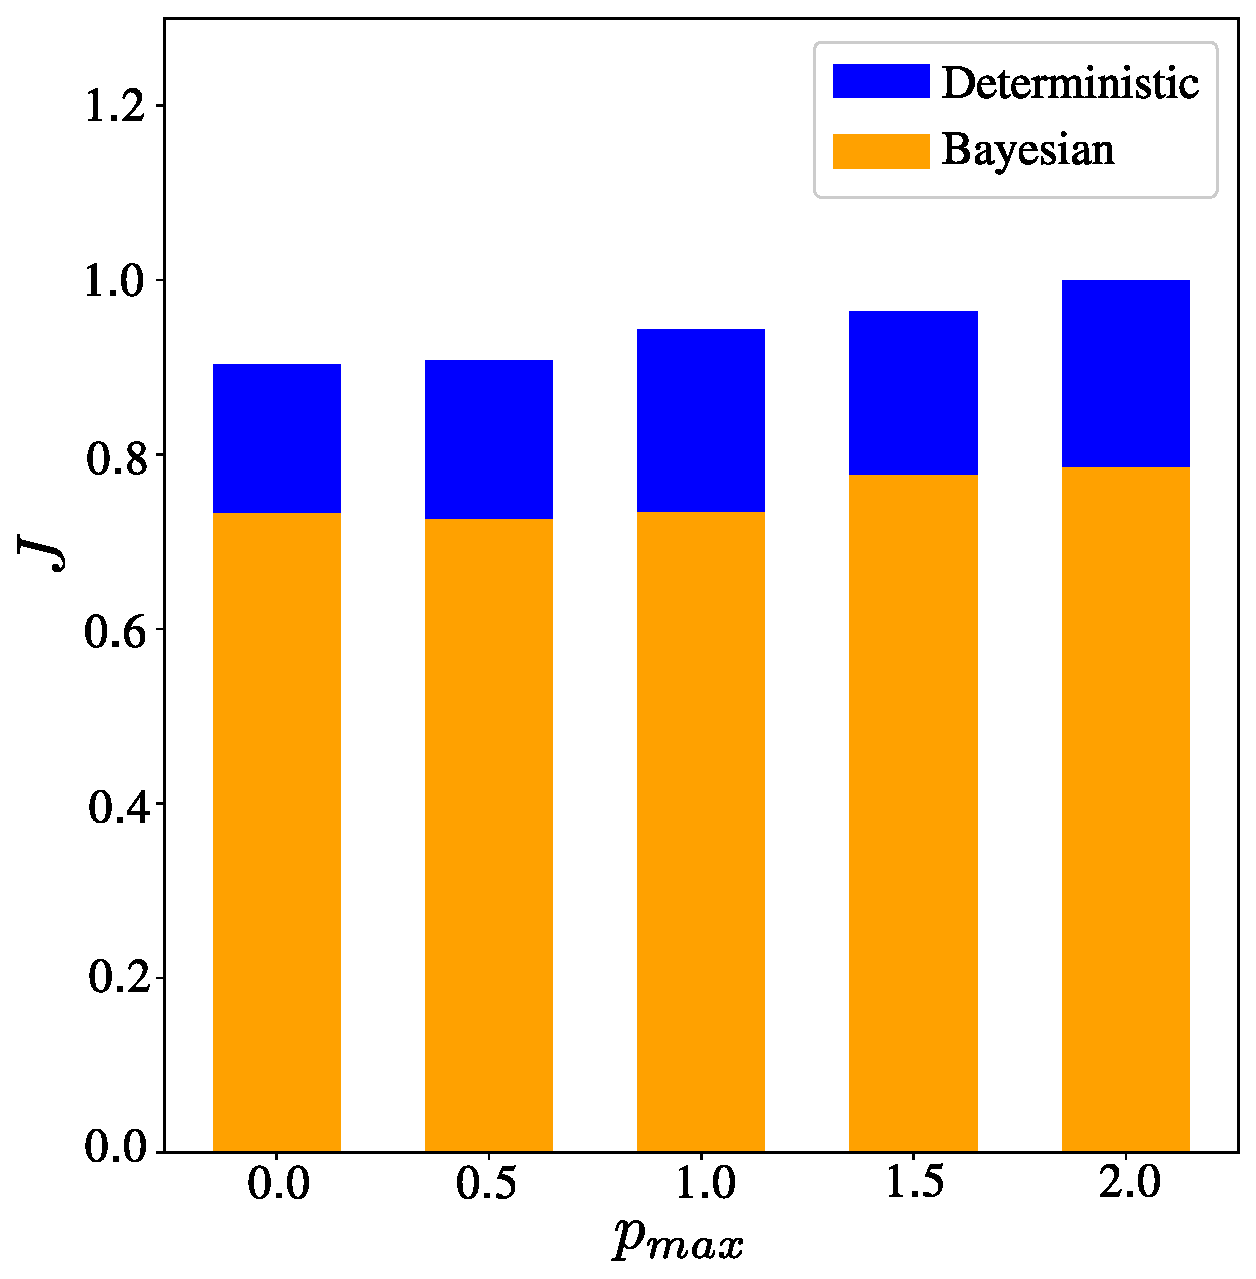
\includegraphics[width=0.7\linewidth]{simulationComparison.eps}
    \label{fig:comparison}
\end{figure}

\subsubsection{Real-World Experiments}

We test the performance of both controllers on the hardware shown in
Figure~\ref{fig:hardware}.
%
The robot consists of two set of $10$ spokes for stability.
%
The torso holds two ODrive v3.6 brushless DC motors, which actuate the drive
shaft through a belt-drive system.
%
The end of the Aluminum spokes land on preloaded springs to reduce vibration,
while the rubber feet ensure no-slip condition.
%
The incremental capacitive encoders attached to the motors report the
orientation of the spokes.
%
We use IMU readings fused with Mahony filter~\cite{mahony2008nonlinear} to estimate
the pitch of the torso.
%
A 24V battery pack is placed at the bottom edge of the torso to power
the motors, a Raspberry Pi 3B and a Teensy microcontroller.
%
We evaluate the neural networks on a laptop and exchange sensor readings and
torque commands with the Raspberry Pi via ROS wireless communication protocols.


\begin{figure}[H]
    \centering
    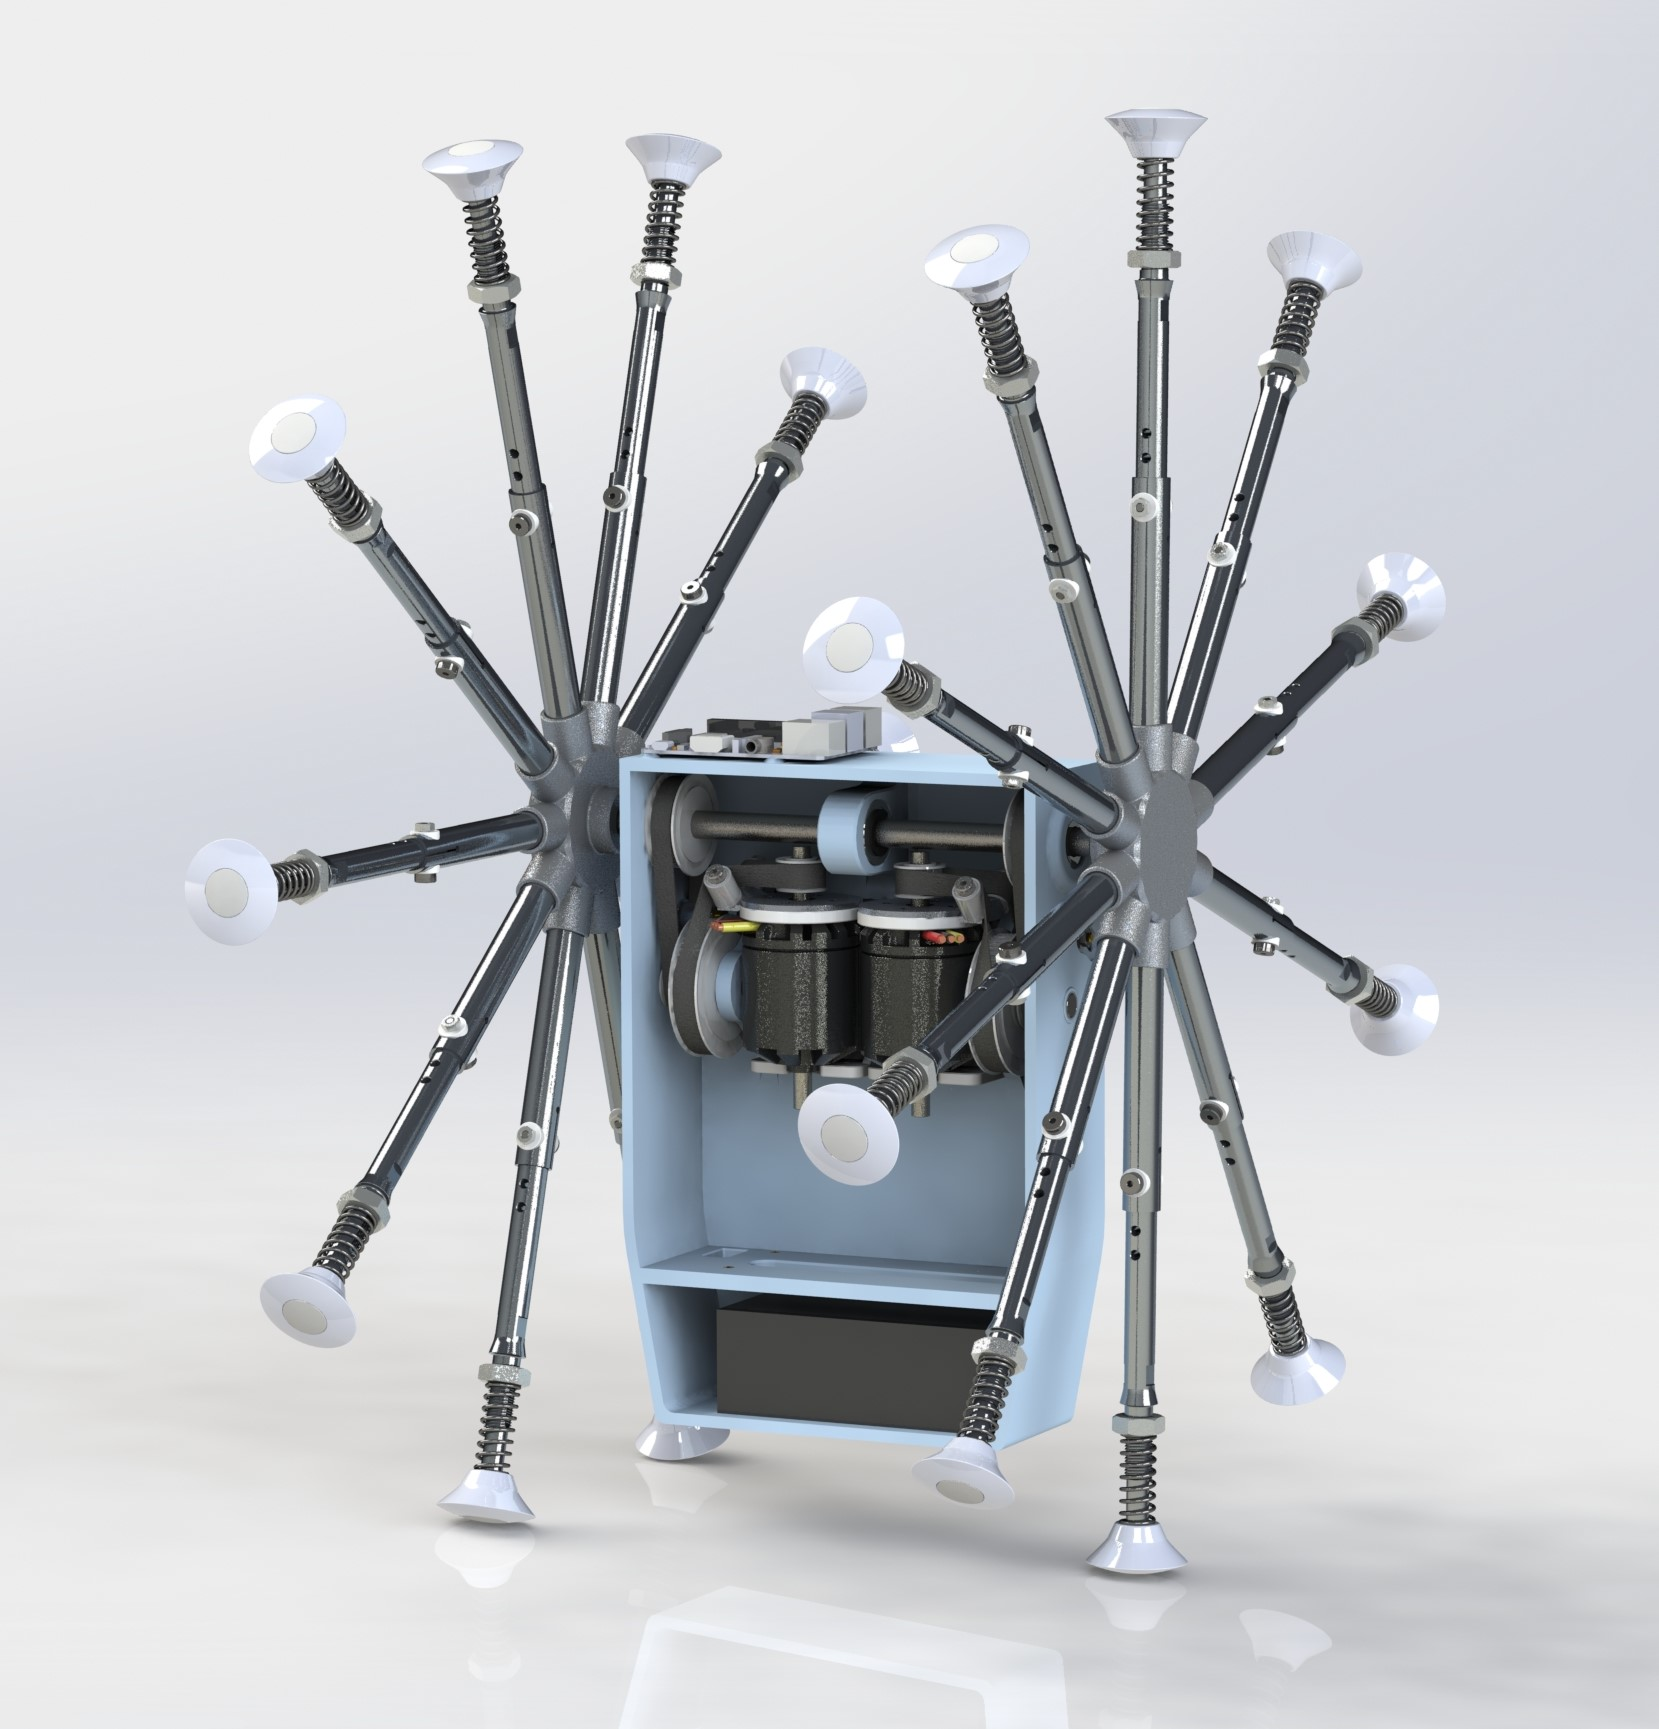
\includegraphics[width=0.7\columnwidth]{rendering.JPG}
    \caption{Rimless Wheel Assembly}
    \label{fig:hardware}
\end{figure}